% Lecture Template for ME3001-001-Tristan Hill - Spring 2020
% Mechanical Engineering Analysis with MATLAB
% Ordinary Differential Equations - Lecture 2

% I am finally converting my stuff to BEAMER

% Document settings



%\documentclass{beamer}                  % for presentation ?
\documentclass[handout]{beamer}  % for handout ?
\usepackage{beamerthemesplit}
\usepackage{amsmath}
\usepackage{listings}
\usepackage{multicol}

\beamertemplateballitem

\definecolor{TTUpurple}{rgb}{0.3098, 0.1607, 0.5176} % TTU Purple (primary)
\definecolor{TTUgold}{rgb}{1.0000, 0.8666, 0.0000} % TTU Gold (primary)

\setbeamercolor{palette primary}{bg=TTUpurple,fg=TTUgold}
\setbeamercolor{palette secondary}{bg=black,fg=TTUgold}
\setbeamercolor{palette tertiary}{bg=black,fg=TTUpurple}
\setbeamercolor{palette quaternary}{bg=TTUgold,fg=black}
\setbeamercolor{structure}{fg=TTUpurple} % itemize, enumerate, etc
\setbeamercolor{section in toc}{fg=TTUpurple} % TOC sections

%\usefonttheme{professionalfonts}

\newcommand{\LNUM}{2\hspace{2mm}} % Lecture Number 
\newcommand{\secondtitle}{Analytical Solutions to Differential Equations}% second line of the title of this presentation , aka the topic of this lecture
\newcommand{\vspcc}{\vspace{6mm}\\ } 
\newcommand{\vspc}{\vspace{3mm}\\ } 
\newcommand{\hspc}{\hspace{5mm} } 


\title{\vspace{2mm}\\Ordinary Differential Equations - Lecture \LNUM}
\author{ME3001 - Mechanical Engineering Analysis} % original formatting from Mike Renfro, September 21, 2004

\date{April 03, 2020}

\begin{document}

\lstset{language=MATLAB,basicstyle=\ttfamily\small,showstringspaces=false}



\frame{\titlepage \center\textbf{\secondtitle}\vspcc}

%\section*{Outlines}
%\subsection*{Part I: Review of Previous Lecture}
%\frame{
%  \nameslide{outline}
%  \frametitle{Review of Previous Lecture}
%  \tableofcontents[part=1]
%}

%\subsection*{Part II: Solution of Simultaneous Linear Algebraic Equations}
%\frame{
%  \frametitle{Solution of Simultaneous Linear Algebraic Equations}
%  \tableofcontents[part=1]
%}

%\part{Review of Previous Lecture}
%\frame{\partpage}

%\frame{
%  \frametitle{Review of Previous Lecture}

%  \begin{itemize}
%  \item<+-| alert@+> Sample problems solved with numerical methods
%    \begin{itemize}
%    \item<+-| alert@+> Natural frequencies of a vibrating bar
%    \item<+-| alert@+> Static analysis of a scaffolding
%    \item<+-| alert@+> Critical loads for buckling a column
%    \item<+-| alert@+> Realistic Design Properties of Materials
%    \end{itemize}
%  \item<+-| alert@+> Solution of nonlinear equations
%    \begin{itemize}
%    \item<+-| alert@+> Introduction
%    \item<+-| alert@+> Example: fluid mechanics
%    \item<+-| alert@+> Incremental search method
%    \end{itemize}
%  \end{itemize}
%}
%ballitem
%\part{Solution of Simultaneous Linear Algebraic Equations}
%\frame{\partpage}

\frame{

{\bf Lecture \LNUM - \secondtitle :} \vspace{3mm}\\ % ' topics' are beamer 'sections' - TWH

 \begin{itemize}
	\item Review\vspace{5mm}\\
	\item Analytical vs. Numerical Methods \vspace{5mm}\\	
	\item Example - Separation of Variables \vspace{5mm}\\

\end{itemize}

}

\section{Review}

\frame{

  \frametitle{What is a Differential Equation? Solution?}

A {\bf differential equation} is an equation which describes a function \vspace{3mm}\\and one or more of its \underline{\hspace{50mm}} of the \vspace{3mm}\\ \underline{\hspace{50mm}}\hspace{3mm}\underline{\hspace{50mm}}\vspace{2mm}\\ with respect to the \underline{\hspace{60mm}}. \vspace{8mm} \\
 
The {\bf solution} to a differential equation describes the \vspace{2mm}\\ \underline{\hspace{40mm}}\hspace{2mm}\underline{\hspace{40mm}} as a function \vspace{2mm}\\of the \underline{\hspace{40mm}}\hspace{2mm}\underline{\hspace{40mm}}.  \vspace{5mm}\\

}


\section{Analytical vs. Numerical Methods}

\subsection{Analytical Method}
\frame{

  \frametitle{Analytical Methods}

 A solution to a problem that can be written in "closed form" in terms of known functions, constants, etc., is often called an {\bf analytic solution}. Note that this use of the word is completely different from its use in the terms analytic continuation, analytic function, etc. \vspace{3mm}\\

{\bf Analytical solutions}, also called closed-form solutions, are mathematical solutions in the form of math expressions. If you are developing algorithms or modeling engineering systems, analytical solutions offer the advantages of transparency and efficiency. 

}

\subsection{Numerical Solutions}
\frame{

  \frametitle{Numerical Solutions}

A {\bf numerical solution} is an approximation to the solution of a mathematical equation, often used where analytical solutions are hard or impossible to find. All numerical solutions are approximations, some better than others, depending on the context of the problem and the numerical method used. \vspace{3mm}\\

{\bf Numerical methods} for ordinary differential equations are methods used to find numerical approximations to the solutions of ordinary differential equations (ODEs). Their use is also known as "numerical integration", although this term is sometimes taken to mean the computation of integrals.

}




\section{Engineering Example - Analytical Solution}
\subsection{Problem Statement}
\frame{

\frametitle{Problem Statement}



Remember our example from the previous lecture?\vspace{5mm}\\

        \scalebox{1.25}{$\dot{v}+\frac{c}{m}v=f(t)$} \vspace{2mm}\\
	
	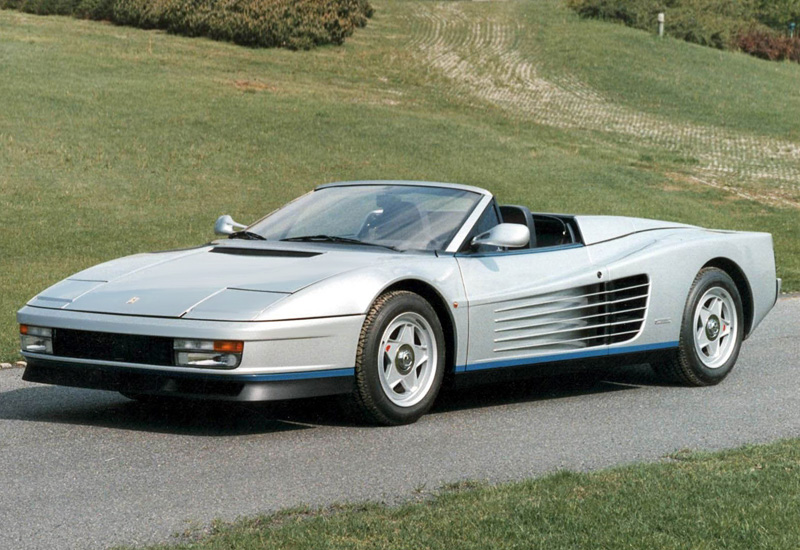
\includegraphics[scale=0.15]{ferrari.jpg} \hspace{10mm} 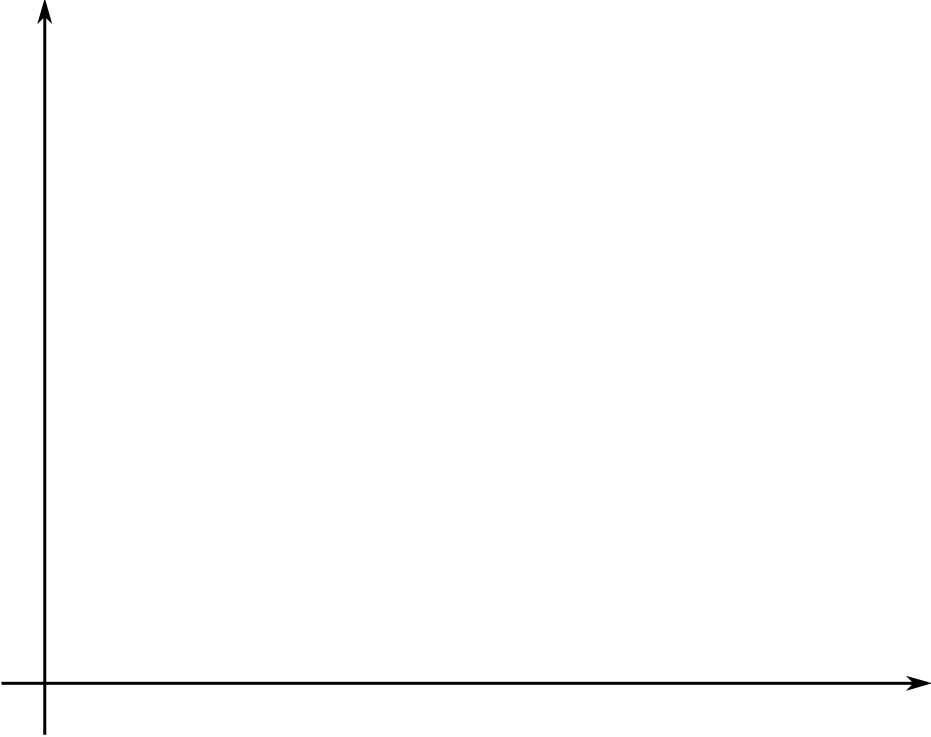
\includegraphics[scale=0.10]{lecture1_fig2.png}\vspace{2mm}\\
	
	
We are going to find an {\bf analytical solution} to this problem. 
  

}

\subsection{Separation of Variables}
\frame{

\frametitle{Separation of Variables}

This is an {\bf analytical} method that you learned in calculus. \vspace{2mm}\\
Assume the external force $f(t)$ is zero. Re-write then separate. \vspace{5mm}\\

\scalebox{1.25}{$\dot{v}+\frac{c}{m}v=0$} \vspace{50mm}\\

}

\subsection{Solution}
\frame{

\frametitle{Solution}

The solution $v(t)$ has been found. What does it mean? What do we do next?\vspace{5mm}\\

\scalebox{1.25}{$v(t)=$} \vspace{50mm}\\


}

\frame{

\frametitle{Graph of Solution}

What does the solution look like?\vspace{5mm}\\
\scalebox{1.25}{$v(t)=v_0e^{-\frac{c}{m}t}$} \vspace{5mm}\\

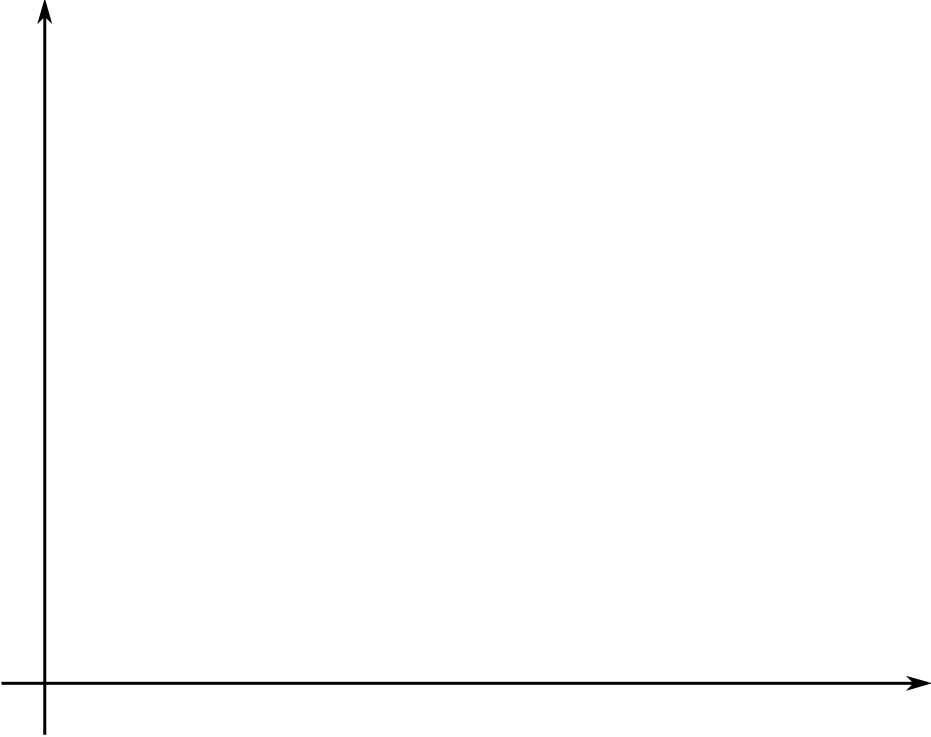
\includegraphics[scale=0.15]{lecture1_fig2.png}\hspace{5mm}%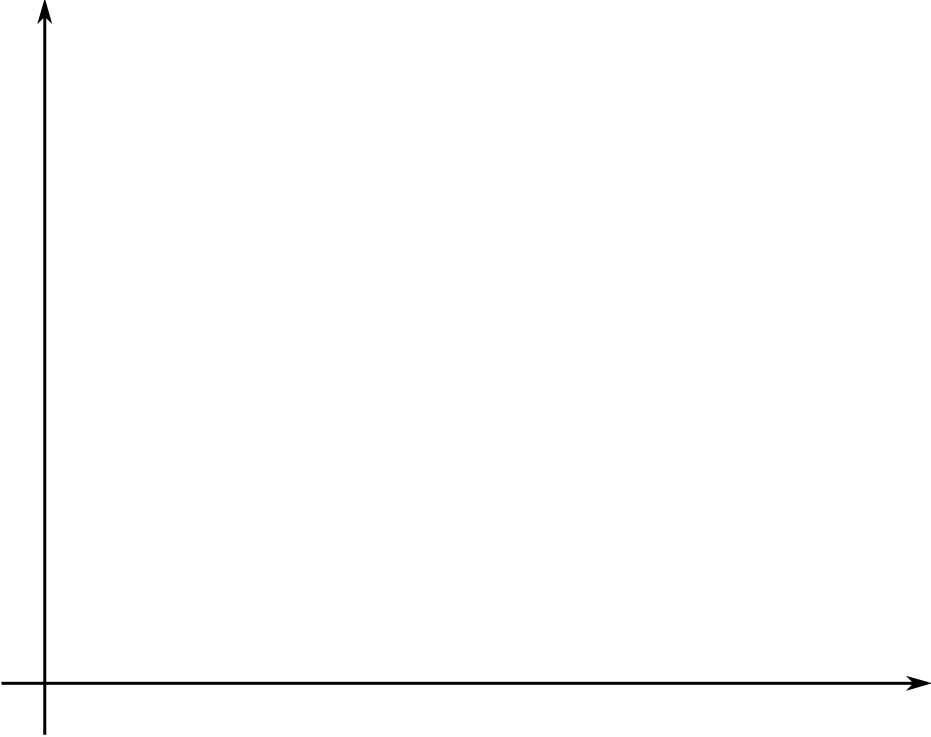
\includegraphics[scale=0.15]{lecture1_fig2.png}

}


\end{document}









